\section{Conjuntos de instancias de prueba}
A lo largo de los años se han propuesto múltiples conjuntos de instancias de prueba para medir el desempeño de los algoritmos para la resolución del JSP. Uno de los más famosos fue propuesto en 1963~\cite{fisher1963} y para una de sus instancias de $10\times 10$ la solución óptima no fue encontrada sino hasta finales de los 80s~\cite{carlier1989}.\\
%
Debido al aumento de poder de cómputo y al desarrollo de mejores métodos de solución se han desarrollado conjuntos de prueba cada vez más desafiantes.
%
En la tabla \ref{tab:benchmark} se muestran en orden cronológico los conjuntos más usados. La mayor parte de ellos ya han sido resueltos casi en su totalidad.\\ 
%
\begin{table}[h]
\centering
\begin{tabular}{@{}cccc@{}}
\toprule
Nombre & \begin{tabular}[c]{@{}c@{}}Rango de tamaños\\ (trabajos$\times$máquinas)\end{tabular} & Número de instancias & \begin{tabular}[c]{@{}c@{}}Instancias sin\\ solución óptima\end{tabular} \\ \midrule
ft ~\cite{fisher1963} & $6\times 6$ - $20\times 5$     & 3  & 0  \\
la ~\cite{lawrence1984resource} & $10\times 5$ - $15\times 15$   & 40 & 0  \\
abz~\cite{adams1988shifting} & $10\times 10$ - $20\times 15$  & 5  & 1  \\
orb~\cite{applegate1991computational} & $10\times 10$                & 10 & 0  \\
swv~\cite{storer1992new} & $20\times 10$ - $50\times 10$  & 20 & 5  \\
yn ~\cite{yamada1992genetic} & $20\times 20$                & 4  & 3  \\
ta~\cite{taillard1993benchmarks}  & $15\times 15$ - $100\times 20$ & 80 & 21 \\ 
dmu~\cite{demirkol1998benchmarks} & $20\times 15$-$50\times 20$  & 80 & 54 \\ \midrule
\end{tabular}
    \caption{Conjuntos de instancias de prueba populares}
    \label{tab:benchmark}
\end{table}
%
En general, para generar un conjunto de instancias de prueba se elige un conjunto de valores para los tamaños de las instancias, una distribución de probabilidad para generar los tiempos de procesamiento de cada operación y se determina una manera de asignar las restricciones de precedencia en cada trabajo.
%
La dificultad de las instancias resultantes depende principalmente de dos factores: el tamaño de la instancia y la forma en la que se eligen las restricciones de precedencia en cada trabajo. Los tiempos de procesamiento de cada operación por lo regular se obtienen de una distribución uniforme.\\
%
Puede aumentarse arbitrariamente el tamaño de las instancias para hacerlas más difíciles aunque estos aumentos en dificultad no necesariamente se deben a que el problema sea fundamentalmente más complicado de resolver.
%
Existen varias formas de elegir las restricciones de precedencia. Como cada trabajo se procesa solamente una vez en cada una de las $m$ máquinas, escoger estas restricciones de precedencia equivale a escoger una permutación ($\sigma_i$) de las $m$ maquinas para cada trabajo. Puede escogerse al azar de entre todas las  permutaciones posibles, pero se ha observado que una forma de hacer una instancia mucho más desafiante es dividir a las máquinas en subconjuntos y escoger una permutación para cada uno de ellos. Esto genera un cuello de botella que aumenta mucho el makespan de las soluciones en general y que genera óptimos locales de muy baja calidad. \\

%
Por ejemplo si las máquinas se dividen en dos subconjuntos de igual tamaño, las restricciones de precedencia se eligen escogiendo una permutación de las primeras $k = \lfloor\frac{m}{2}\rfloor$ y concatenando una permutación de las restantes de la forma $\sigma_i = (\sigma_{i0}(0,1,\dots,k),\sigma_{i1}(k+1,k+2,m))$.\\
%
En la figura \ref{fig:bottleneck} podemos observar un caso simple de esto para 5 trabajos ($n=5$) y dos máquinas ($m=2$) en el que la operación inicial de cada trabajo debe procesarse en la misma máquina.\\
%
\begin{figure}[h]
\begin{subfigure}{\textwidth}
    \centering
    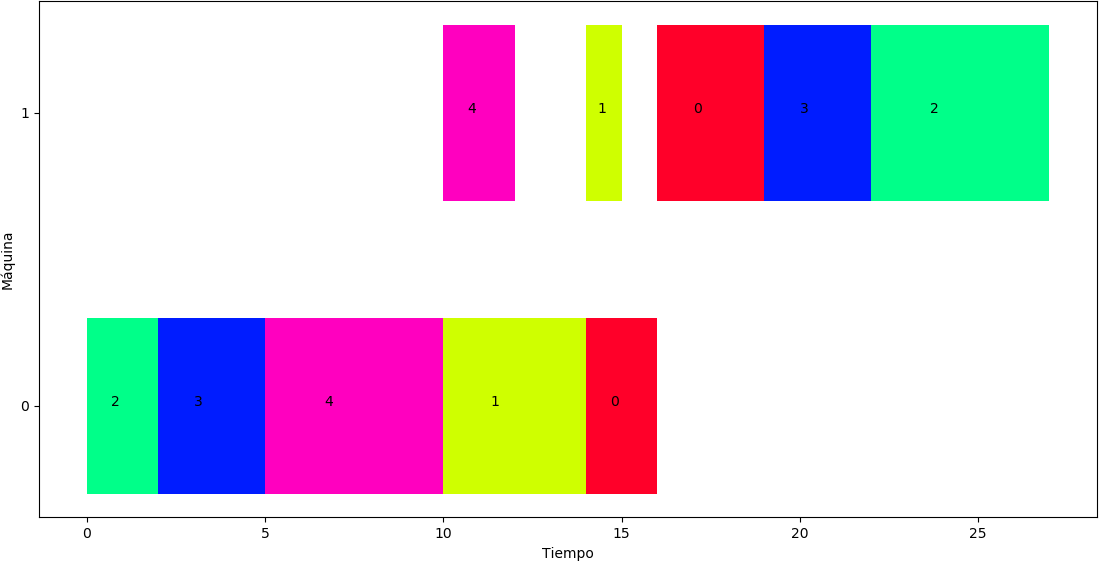
\includegraphics[scale=.5]{Imagenes/casoextremomalo.png}
    \caption{Planificación aleatoria}
\end{subfigure}
\begin{subfigure}{\textwidth}
    \centering
    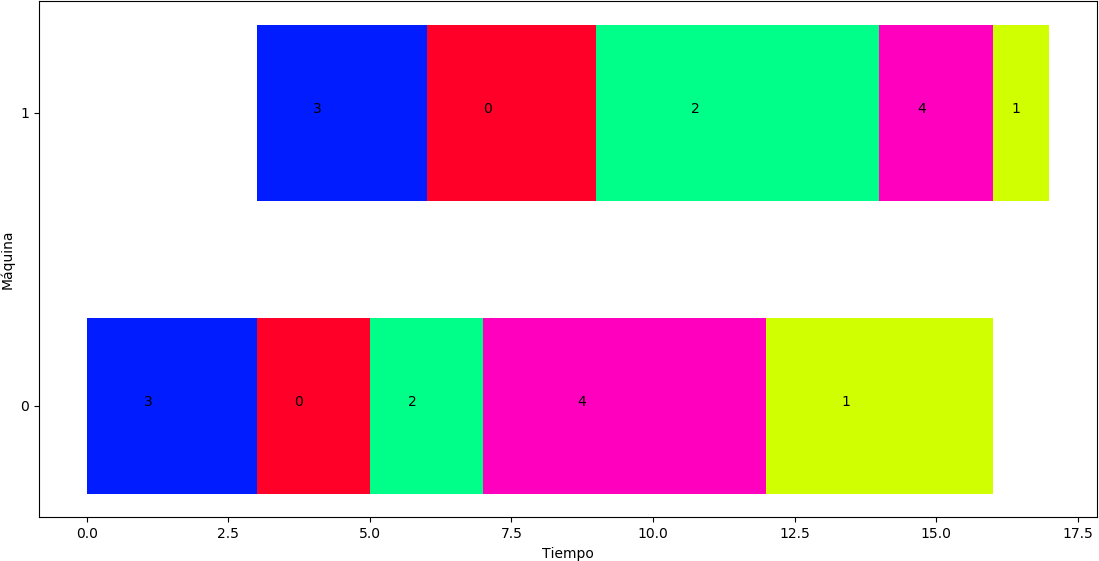
\includegraphics[scale=.5]{Imagenes/casoextremobueno.png}
    \caption{Planificación óptima}
\end{subfigure}
\caption{Ejemplo de planificación para una instancia en la cuál todos los trabajos empiezan en la misma máquina}
\label{fig:bottleneck}
\end{figure}

%
Actualmente el conjunto más popular y reciente es el llamado dmu\cite{demirkol1998benchmarks} también conocido como \textbf{DMU01-80}. La segunda mitad de estas instancias \textbf{DMU40-80} son consideradas especialmente difíciles porque siguen el esquema antes mencionado en el que todos los trabajos tienen operaciones iniciales en la misma mitad de las máquinas. Este conjunto es el que se eligió para probar las propuestas presentadas en este trabajo.

